
%导言区
\documentclass{article}%book,report,letter

\usepackage{ctex}
\usepackage{fontspec}
%\usepackage{color}
%\usepackage{graphicx} %use graph format
%\usepackage{subfigure}
%\usepackage{epstopdf} %eps图片
\usepackage{amsmath}  %字体加粗
%\usepackage{math}
\usepackage{amsthm}
\usepackage{amssymb} %因为所以符号
\usepackage{caption}
\captionsetup[table]{labelsep=space}

%制作页眉页脚
\usepackage{fancyhdr}  
\pagestyle{fancy}  
\lhead{第七周作业}  
\chead{微分方程数值解法}  
\rhead{桑明达 15300180062}  
\lfoot{}  
\cfoot{\thepage}  
\rfoot{}  
\renewcommand{\headrulewidth}{0.4pt}  
\renewcommand{\footrulewidth}{0.4pt} 

%标题
\author{names}
\title{\heiti 微分方程数值解法\\ [2ex] \begin{large} 第七周作业 \end{large}}
\author{\kaishu 桑明达 15300180062}
\date{\today}

% 正文区
\begin{document}
\maketitle

%\newpage

\section{P118 1 $\frac{\mathrm{d}x}{\mathrm{d}t}=\lambda \left ( -u+cos\left ( t \right ) \right )$}

\begin{proof}
	
	(1) $ u \left ( t \right ) $的精确表达式是
	
\begin{align*}
	u\left ( t \right ) = & \frac{1}{e^{\lambda t}}\left ( \int e^{\lambda t}\lambda cos\left ( t \right ) \mathrm{d}t +C \right ) \\
	= & \frac{\lambda }{1+\lambda ^{2}}\left ( sin\left ( t \right ) +\lambda cos\left ( t \right ) \right )+C e^{-\lambda t} \\
\end{align*}

$u\left ( 0 \right )=0$时,$C=-\frac{\lambda ^{2}}{1+\lambda ^{2}}$

$u\left ( 0 \right )=1$时,$C=-\frac{1}{1+\lambda ^{2}}$

\par
    (2) 图1到图4,是$u\left ( 0 \right )=0$情形,图5到图8,是$u\left ( 0 \right )=1$情形。
   
\par
    (3)图9、图10,是$u\left ( 0 \right )=0$情形,图10、图11,是$u\left ( 0 \right )=1$情形。
    
    从图9、图11中可以看出,Gear格式在$\lambda =1000$时,保持了数值稳定。
    
    而从图10、图12中可以看出,Adams格式在$\lambda =1000$时,误差很大,呈指数增长。
    
    
    \begin{figure}
    	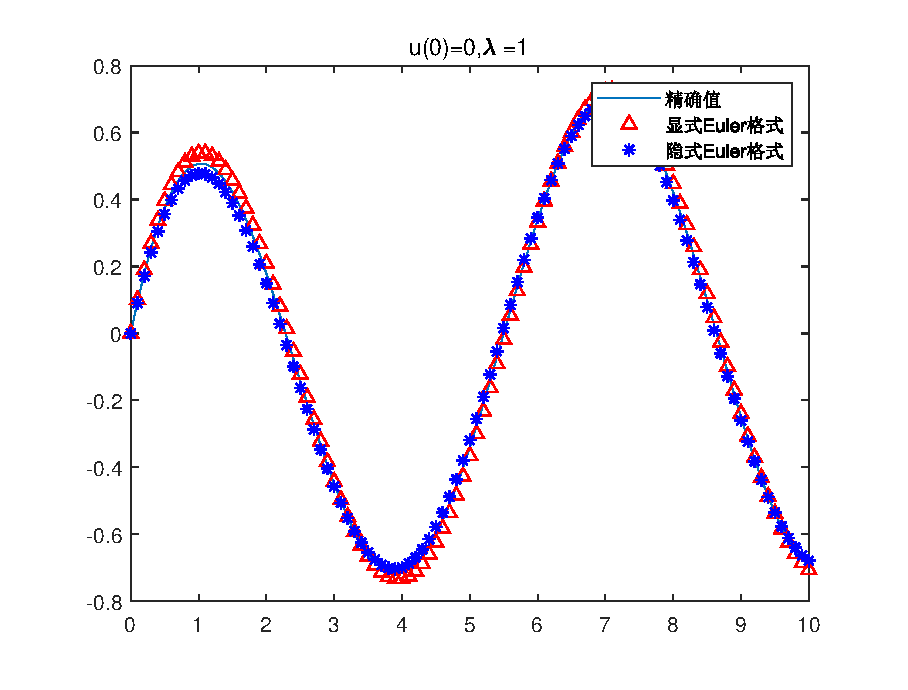
\includegraphics[width=1\linewidth]{pic/week7_1_1.eps}
    	\label{Fig:1}
    	\caption{} 
    \end{figure}
\begin{figure}
	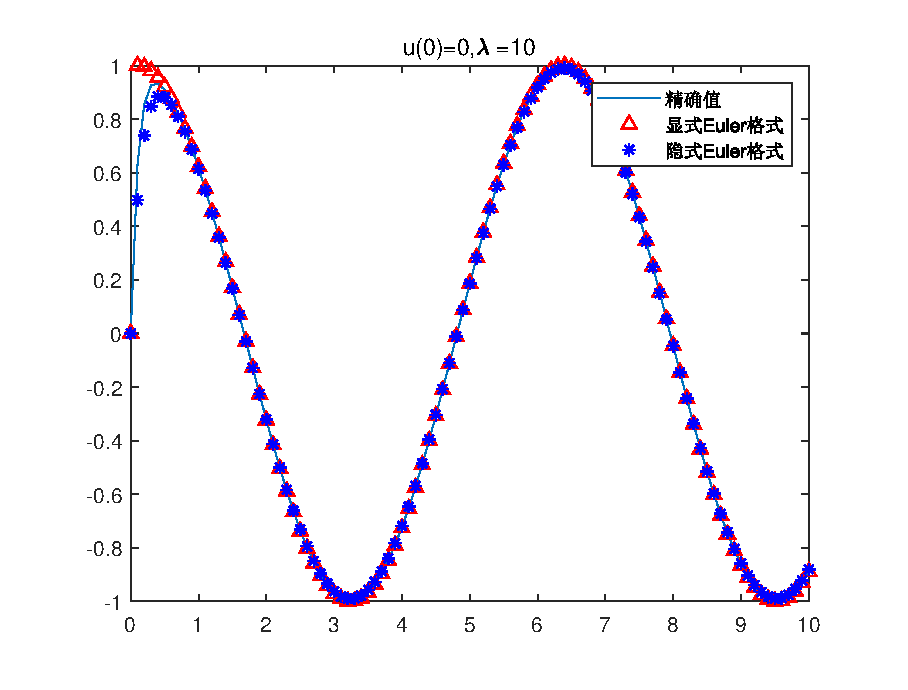
\includegraphics[width=1\linewidth]{pic/week7_1_2.eps}
	\label{Fig:2}
	\caption{} 
\end{figure}
\begin{figure}
	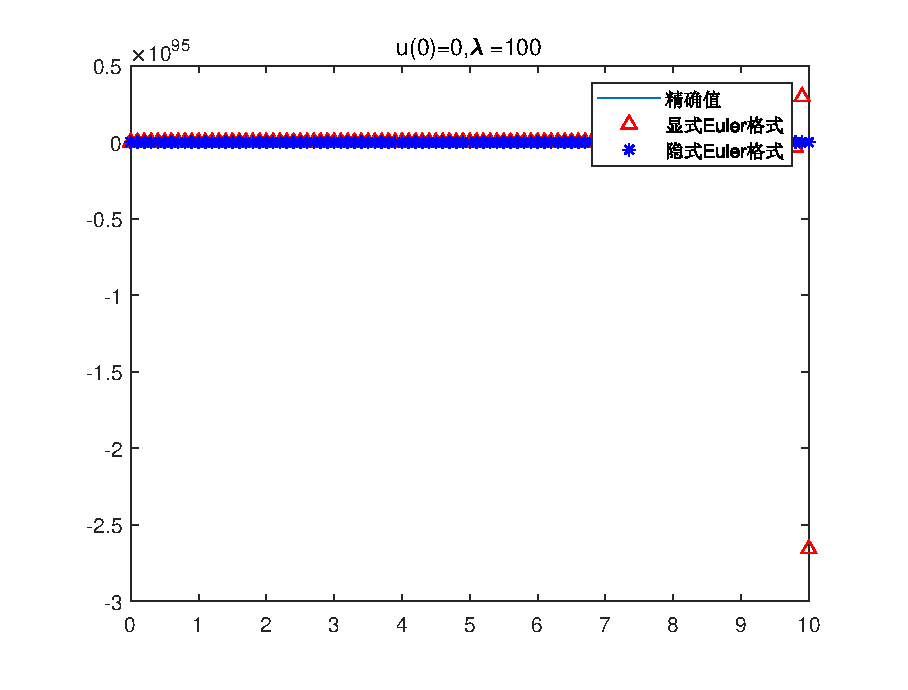
\includegraphics[width=1\linewidth]{pic/week7_1_3.eps}
	\label{Fig:3}
	\caption{} 
\end{figure}
\begin{figure}
	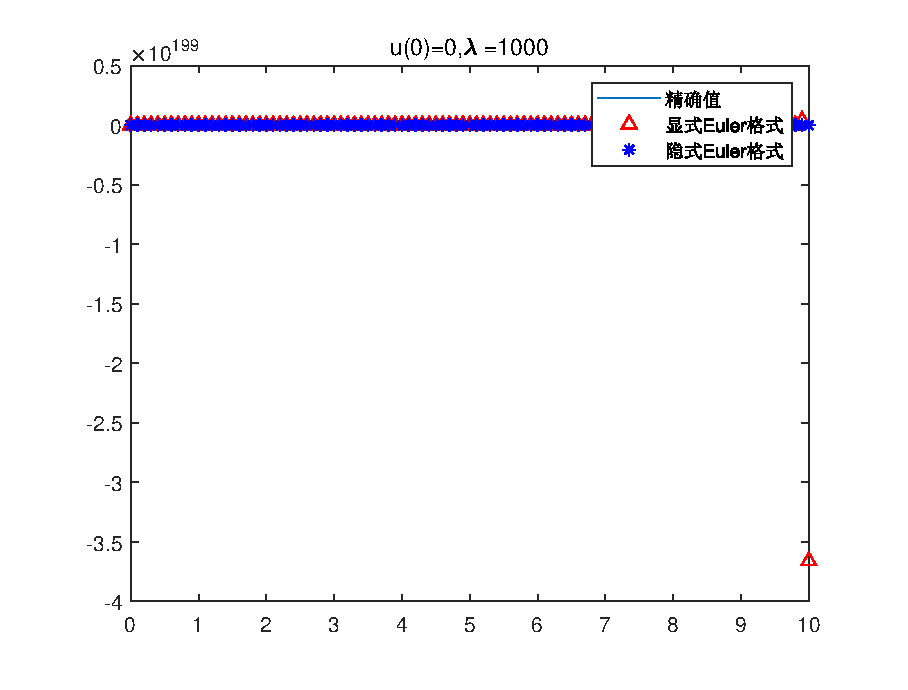
\includegraphics[width=1\linewidth]{pic/week7_1_4.eps}
	\label{Fig:4}
	\caption{} 
\end{figure}
\begin{figure}
	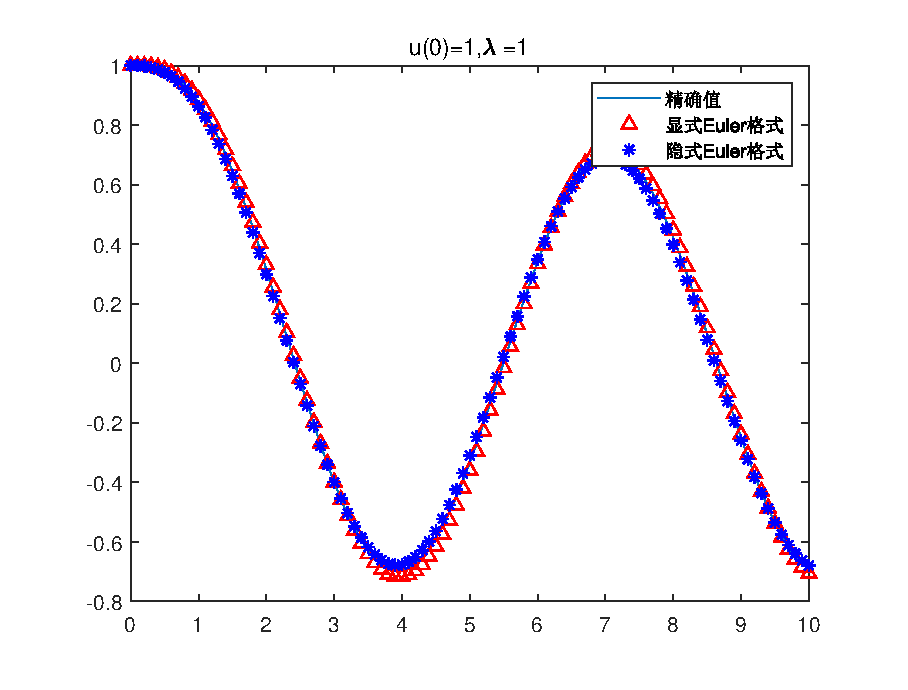
\includegraphics[width=1\linewidth]{pic/week7_1_5.eps}
	\label{Fig:5}
	\caption{} 
\end{figure}
\begin{figure}
	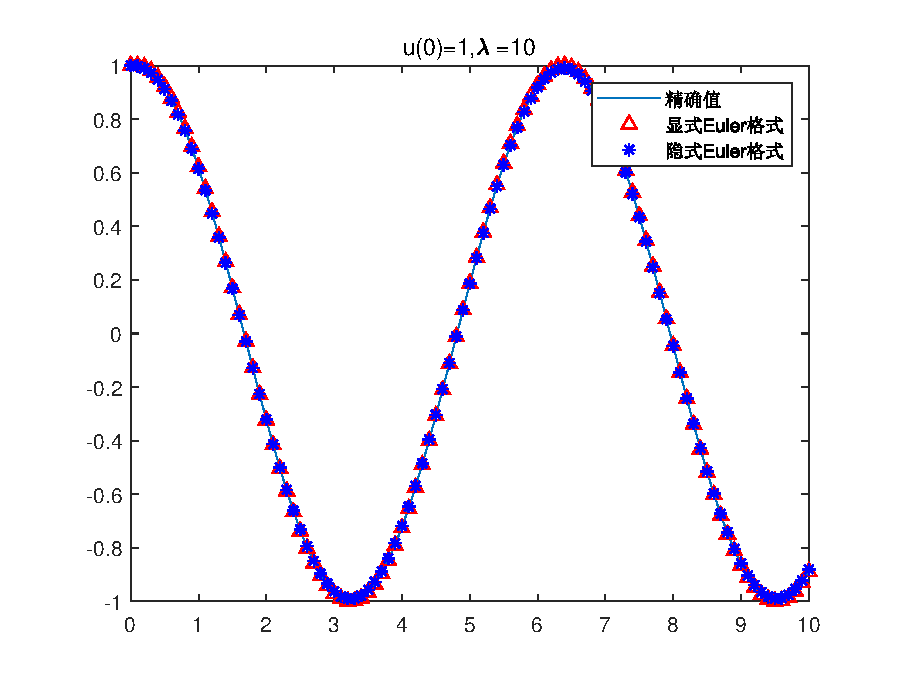
\includegraphics[width=1\linewidth]{pic/week7_1_6.eps}
	\label{Fig:6}
	\caption{} 
\end{figure}
\begin{figure}
	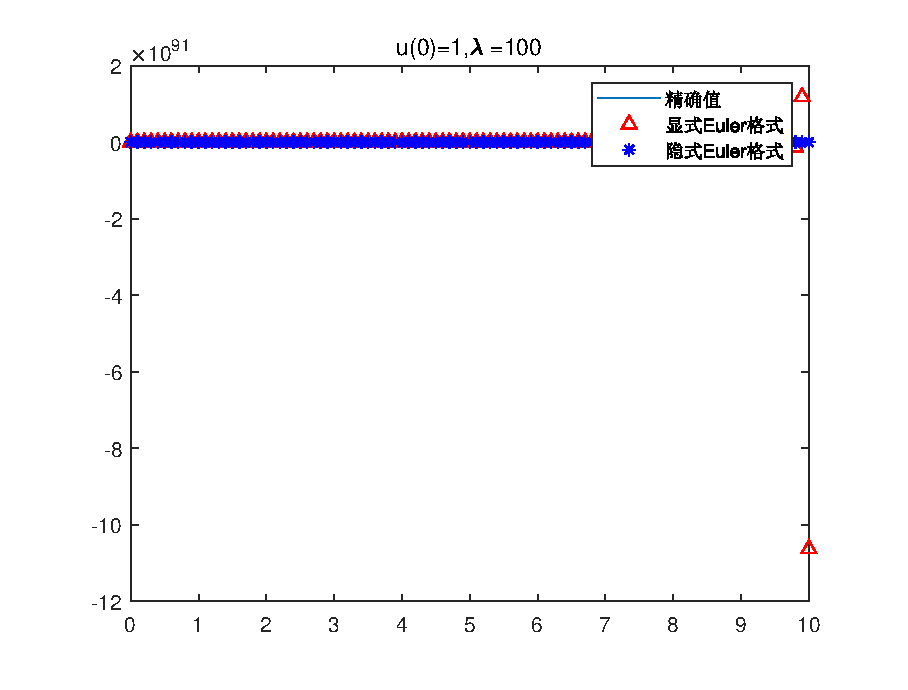
\includegraphics[width=1\linewidth]{pic/week7_1_7.eps}
	\label{Fig:7}
	\caption{} 
\end{figure}
\begin{figure}
	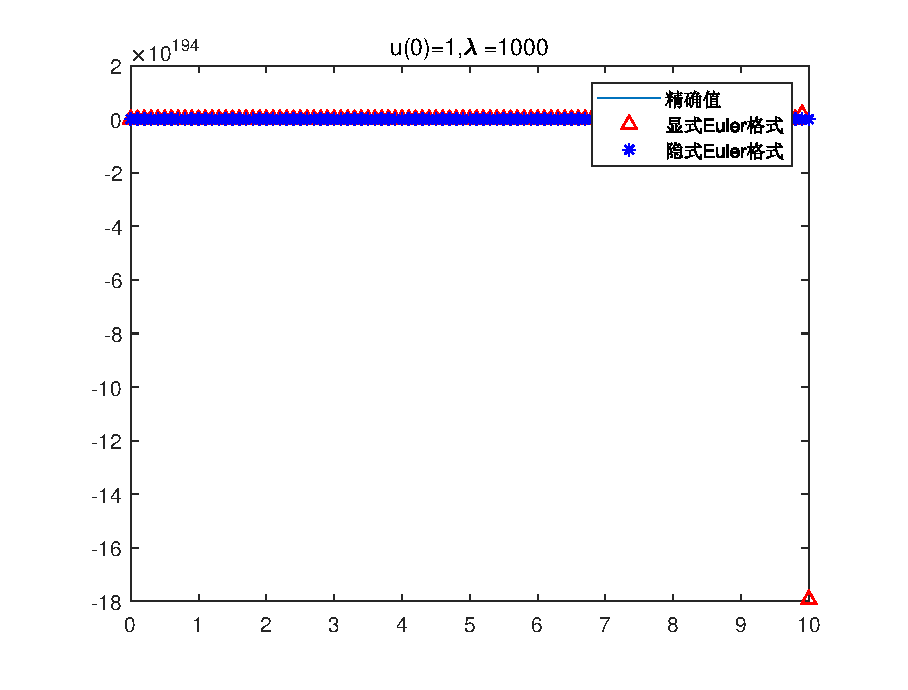
\includegraphics[width=1\linewidth]{pic/week7_1_8.eps}
	\label{Fig:8}
	\caption{} 
\end{figure}
\begin{figure}
	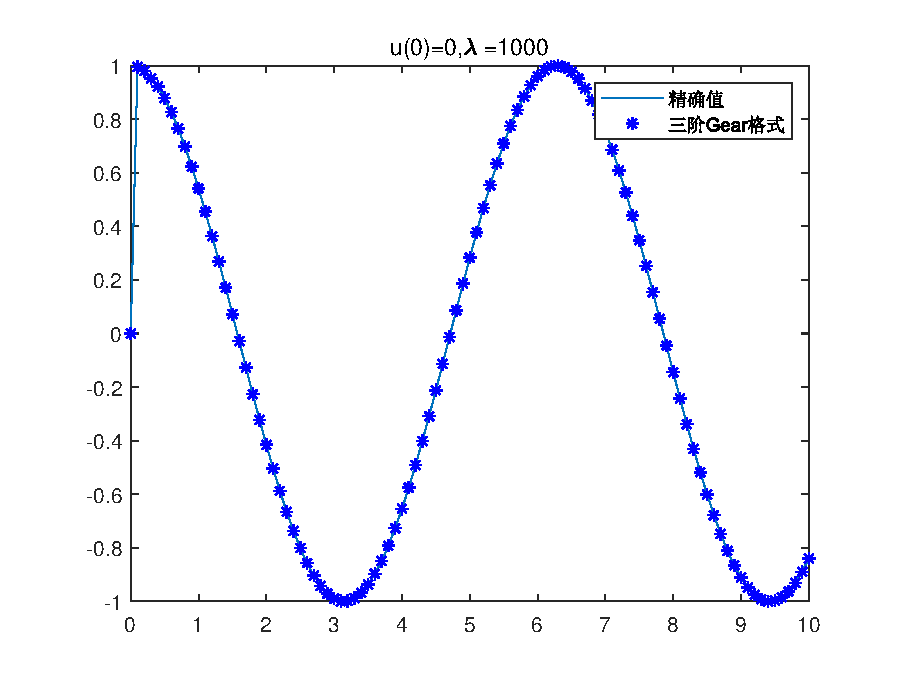
\includegraphics[width=1\linewidth]{pic/week7_1_9.eps}
	\label{Fig:9}
	\caption{} 
\end{figure}
\begin{figure}
	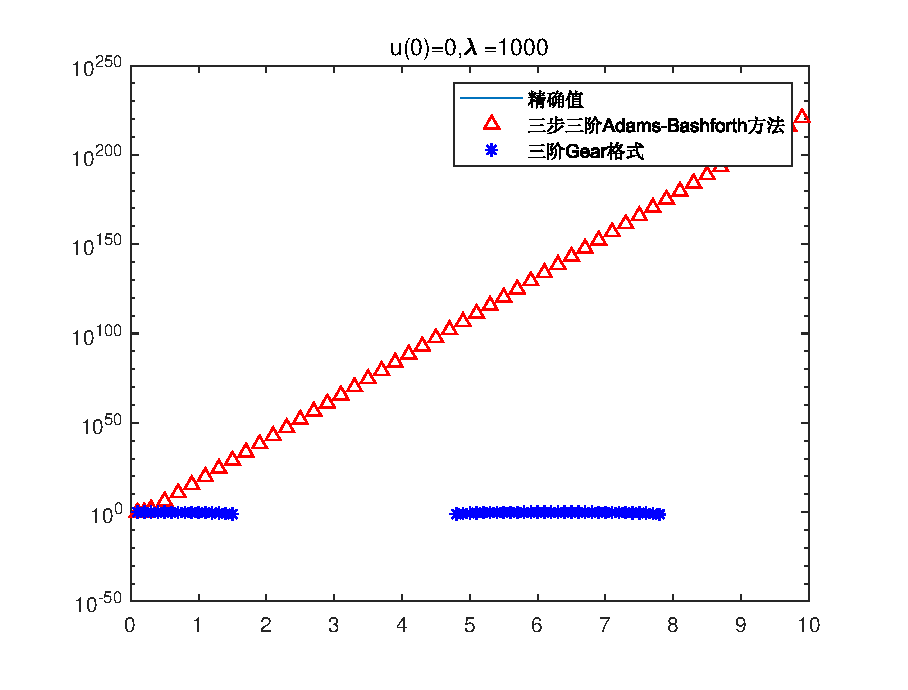
\includegraphics[width=1\linewidth]{pic/week7_1_10.eps}
	\label{Fig:10}
	\caption{} 
\end{figure}
\begin{figure}
	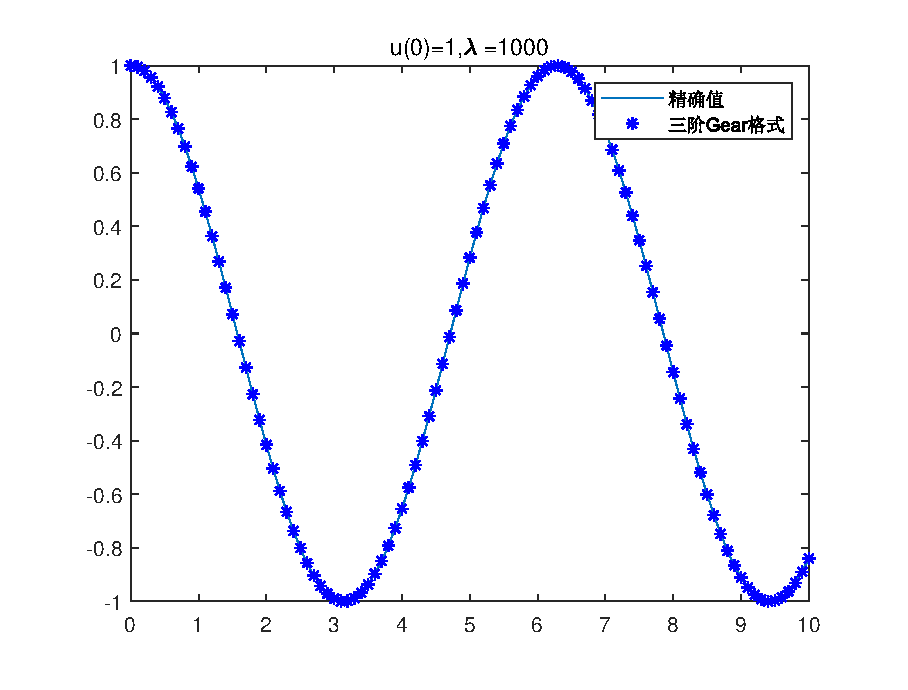
\includegraphics[width=1\linewidth]{pic/week7_1_11.eps}
	\label{Fig:11}
	\caption{} 
\end{figure}
\begin{figure}
	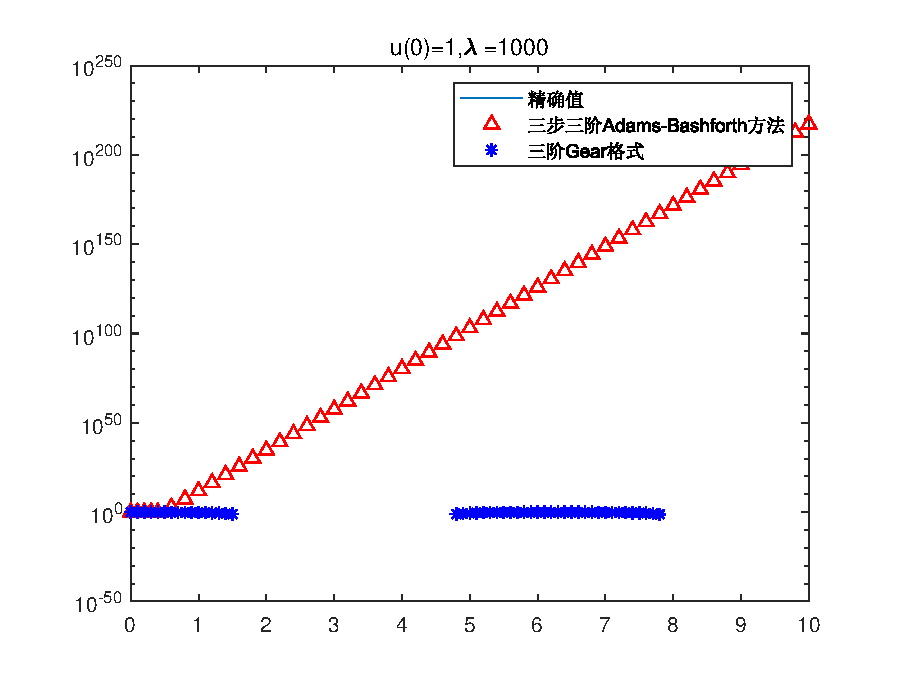
\includegraphics[width=1\linewidth]{pic/week7_1_12.eps}
	\label{Fig:12}
	\caption{} 
\end{figure}

	
	
\end{proof}

\end{document}